\documentclass[11pt,a4paper]{article}

\usepackage{fontspec}
\usepackage{xeCJK}
\setmainfont{DejaVu Serif}
\setsansfont{DejaVu Sans}
\setmonofont{DejaVu Sans Mono}
\setCJKmainfont[AutoFakeBold=2]{Droid Sans Fallback}
\setCJKsansfont[AutoFakeBold=2]{Droid Sans Fallback}
\setCJKmonofont[AutoFakeBold=2]{Droid Sans Fallback}

\usepackage[a4paper,margin=2.15cm]{geometry}
\usepackage{amsmath,amssymb,bm,mathtools}
\usepackage{booktabs,tabularx,longtable,multirow,array}
\usepackage{graphicx,xcolor}
\usepackage{tikz}
\usetikzlibrary{arrows.meta,positioning,fit,calc,shapes.geometric,backgrounds}
\usepackage{float}
\usepackage{enumitem}
\usepackage{caption}
\usepackage{subcaption}
\usepackage{pdflscape}
\usepackage{microtype}
\usepackage{url}
\usepackage{xurl}
\usepackage{hyperref}
\usepackage[nameinlink,noabbrev]{cleveref}
\usepackage{fancyhdr}
\usepackage{listings}

\hypersetup{
  colorlinks=true,
  linkcolor=blue!55!black,
  citecolor=green!35!black,
  urlcolor=blue!65!black,
  pdftitle={From Offline Unified Speech Modeling to Causal Incremental Generation},
  pdfauthor={Jason Lee (Li Jin)}
}

\definecolor{offlineblue}{RGB}{41,98,160}
\definecolor{streamgreen}{RGB}{46,125,50}
\definecolor{futureorange}{RGB}{230,126,34}
\definecolor{frozen}{RGB}{235,238,241}
\definecolor{trainable}{RGB}{220,242,220}

\newcommand{\vect}[1]{\bm{#1}}
\newcommand{\mat}[1]{\bm{#1}}
\newcommand{\R}{\mathbb{R}}
\newcommand{\Vocab}{\mathcal{V}}
\newcommand{\Loss}{\mathcal{L}}
\newcommand{\E}{\mathbb{E}}
\newcommand{\KL}{D_{\mathrm{KL}}}
\newcommand{\checked}{\textcolor{streamgreen}{\ensuremath{\checkmark}}}
\newcommand{\failed}{\textcolor{red!70!black}{\ensuremath{\times}}}

\newcolumntype{Y}{>{\raggedright\arraybackslash}X}
\newcolumntype{C}{>{\centering\arraybackslash}X}
\renewcommand{\arraystretch}{1.16}
\setlength{\tabcolsep}{5pt}
\setlength{\emergencystretch}{2em}
\setlist{nosep,leftmargin=2em}
\captionsetup{font=small,labelfont=bf}

\pagestyle{fancy}
\fancyhf{}
\lhead{UniSS Offline--Streaming S2ST Technical Report}
\rhead{August 25, 2026}
\cfoot{\thepage}
\setlength{\headheight}{14pt}

\lstset{
  basicstyle=\ttfamily\small,
  breaklines=true,
  frame=single,
  backgroundcolor=\color{gray!5},
  columns=fullflexible
}

\title{\textbf{From Offline Unified Speech Modeling to Causal Incremental Generation: \\
UniSS Phase 1--3, Streaming Stage A/B, and a Quality-Aware Reinforcement Learning Route}}
\author{Jason Lee (Li Jin)\\
\small UniSS Training Reproduction and Simultaneous S2ST Project}
\date{August 25, 2026}

\begin{document}
\maketitle

\begin{abstract}
This report presents a complete engineering and research route for extending an offline speech-to-speech translation (S2ST) system into a streaming or simultaneous S2ST system. The offline model uses Qwen2.5-0.5B-Instruct as a shared autoregressive backbone and represents text, GLM acoustic tokens, and BiCodec semantic tokens in a unified vocabulary. Training proceeds through Phase 1 foundational multitask alignment, Phase 2 direct S2ST with capability replay, and Phase 3 Quality/Performance specialization. The public UniST-198 reproduction contains 19,785,924 training records. The best Phase 3 checkpoint reaches Quality-mode Chinese-to-English/English-to-Chinese Text-BLEU scores of 39.38/48.17 and Speech-BLEU scores of 22.73/46.31 on the UniST test set. Relative to Phase 2, Phase 3 improves 21 of 24 principal higher-is-better test cells.

The streaming route preserves the successful Phase 3 architecture and introduces two causal adaptation stages. Stage A connects a chunk-causal WhisperVQ frontend and an acoustic bridge to the shared Qwen model to learn append-only streaming ASR. Its 381-update training run is numerically stable, but its free-running weighted WER/CER remains 27.14\%, so the formal quality gate is not passed. Stage B freezes the Stage A causal acoustic frontend and updates only the shared Qwen at a low learning rate using five task families: streaming ASR, incremental MT, end-to-end semantic deltas, and two Phase 3 replay modes. Stage B completes 2,264 updates. For English-to-Chinese at 160/320\,ms decision chunks, it reduces first translated audio from 4.22\,s to 2.40/2.88\,s, corresponding to improvements of 1.82/1.34\,s. These early outputs are nevertheless incomplete, while Chinese-to-English degrades because an incorrect irreversible ASR prefix propagates through MT and speech synthesis. We therefore do not claim that Stage B is a bidirectional overall success.

Building on these findings, we formulate a future quality-aware Group Relative Policy Optimization (GRPO) stage. For each input, the policy samples multiple READ/WRITE--content--audio trajectories and receives a reward combining final translation quality, prefix support, First WRITE, average token delay, completeness, non-silence, and boundary continuity, with reference-policy KL regularization. Earlier action-only GRPO experiments show why this extension is needed: a group-size-8 policy improves Chinese-to-English Text-BLEU by 1.87 over matched continued SFT, but increases First WRITE by 41.85\,ms. Reward-v2 experiments provide preliminary evidence that bilingual quality terms and adaptive KL can reduce ATD by 24.7--46.5\,ms without necessarily sacrificing both directions. The principal contributions of this work are a reproducible unified-token offline curriculum, Phase-3-anchored causal acoustic adaptation, trajectory-routed joint incremental training in a single shared decoder, and an evaluation framework that explicitly separates verified gains, failed gates, proxy latency, and proposed reinforcement learning.
\end{abstract}

\noindent\textbf{Keywords:} speech-to-speech translation; simultaneous translation; streaming ASR; incremental machine translation; speech tokens; multitask learning; GRPO; quality--latency trade-off

\section{Introduction}

Direct speech-to-speech translation aims to map the linguistic content, language, and expressive characteristics of source speech into target-language speech. An offline system may observe the complete utterance before planning the translation and target waveform. A simultaneous system must instead make irreversible decisions before the future source context is available. Let the 16-kHz source waveform be the vector $\vect{s}\in\R^{N}$, where $N$ is the number of samples and $N/16000$ is the duration in seconds. An offline system estimates $p_\theta(\vect{y}\mid\vect{s})$, where $\vect{y}=(y_1,\ldots,y_L)\in\Vocab^L$ is a target token sequence of length $L$ and $\Vocab$ is the unified vocabulary. At arrival event $k$, a streaming system may only access the prefix $\vect{s}_{1:n_k}\in\R^{n_k}$ and must emit an append-only increment $\Delta\vect{y}_k$. Previously emitted increments may not be revised. This creates three coupled conflicts: insufficient evidence versus premature output, waiting versus interaction latency, and fragmented generation versus speech continuity.

Our offline foundation follows the unified expressive S2ST formulation of UniSS\cite{cheng2025uniss}. It uses a Qwen2.5\cite{yang2024qwen25} Transformer to model text, source speech representations, and target BiCodec semantic tokens in a single autoregressive space. Training is implemented with Megatron-LM\cite{shoeybi2019megatron} and covers all 198 public UniST training shards. The streaming route draws on the READ/WRITE abstraction of prefix-to-prefix and wait-$k$ translation\cite{ma2019stacl} and on the multitask, multi-chunk motivation of StreamSpeech\cite{zhang2024streamspeech}, while deliberately retaining the successful Phase 3 architecture and codec.

This work addresses four empirical questions:

\begin{enumerate}
  \item Can a shared 0.5B autoregressive model reliably acquire ASR, translation, and speech-generation capabilities through a Phase 1--3 curriculum on the full public dataset?
  \item Can a chunk-causal acoustic frontend support append-only streaming ASR without discarding the best Phase 3 checkpoint?
  \item After freezing that frontend, can the shared Qwen jointly learn ASR deltas, incremental translation deltas, and target semantic deltas while retaining offline capabilities?
  \item Can trajectory-level reinforcement learning improve the quality--latency trade-off that supervised trajectory learning does not optimize directly?
\end{enumerate}

The main technical contributions are as follows.

\begin{itemize}
  \item \textbf{A three-phase offline curriculum in a unified token space.} Text, GLM acoustic tokens, and BiCodec semantic tokens are modeled by the same 24-layer, 896-dimensional Qwen backbone. Phase 2 uses a 2:1 mixture of new tasks and Phase 1 replay, followed by Phase 3 Quality/Performance specialization. Phase 3 improves 21 of 24 principal test cells over Phase 2.
  \item \textbf{Phase-3-anchored causal acoustic transfer.} Stage A does not train a separate streaming system from scratch. It inserts a chunk-causal WhisperVQ frontend and bridge into the Phase 3 model and retains exact Phase 3 replay, making the origin of causal adaptation and capability retention auditable.
  \item \textbf{Five-family incremental training in one shared decoder.} Stage B combines streaming ASR, incremental MT, interleaved S2ST semantic deltas, and two Phase 3 replay modes in a globally synchronized schedule. Gold and free-running histories, alignment confidence, and clean/noisy/quarantine strata control supervision reliability.
  \item \textbf{Completeness-aware END margin and commit consistency.} A logit margin discourages premature semantic END, while a consistency term protects already committed prefixes. The resulting English-to-Chinese first-audio improvement is measurable, but the failed Chinese-to-English gate reveals the cost of aggressive irreversible commits.
  \item \textbf{A quality-aware trajectory-level RL formulation.} Rather than optimizing only a binary WAIT/WRITE head, the proposed reward jointly measures final text and speech quality, prefix safety, latency, completeness, non-silence, and audio continuity. We state matched-SFT and Pareto-frontier criteria that must be met before an RL gain can be claimed.
\end{itemize}

\section{Related Work}

\subsection{Unified Expressive Speech-to-Speech Translation}

UniSS represents source acoustics, intermediate text, and target speech semantics in a unified language-model vocabulary, with Quality and Performance protocols providing different generation paths\cite{cheng2025uniss}. Our Offline Phase 1--3 is a public-data, 0.5B reproduction of this principle; it is not an exact reproduction of the original 1.5B model and its complete training corpus. Whisper provides a strong acoustic representation through large-scale weak supervision\cite{radford2022whisper}. Qwen2.5 supplies the shared autoregressive language-model backbone\cite{yang2024qwen25}. BiCodec/Spark-TTS-style decoupling of global speaker tokens and local semantic tokens supports target speech generation in the source speaker's voice\cite{wang2025sparktts}.

\subsection{Streaming Translation and Simultaneous S2ST}

STACL formulates simultaneous translation as prefix-to-prefix generation and uses wait-$k$ to control latency\cite{ma2019stacl}. A fixed policy is simple but cannot adapt its waiting behavior to the ambiguity of a particular source prefix. StreamSpeech combines a streaming encoder, multitask learning, multi-chunk training, and CTC-based counting of source and target units\cite{zhang2024streamspeech}. We adopt its motivations that one model should cover multiple latency operating points and that ASR/MT auxiliary objectives should protect end-to-end S2ST. We do not directly reproduce its non-autoregressive unit CTC decoder: target speech remains a sequence of BiCodec semantic tokens generated by the Phase 3 autoregressive LM head.

\subsection{Reinforcement Learning for Group-Relative Trajectory Optimization}

GRPO estimates a normalized relative advantage from multiple responses to the same input, avoiding a separately trained value critic and constraining the learned policy with reference-policy KL\cite{shao2024deepseekmath}. This is relevant to simultaneous S2ST because automatically generated trajectories provide only one approximate READ/WRITE target, whereas the actual objective is a Pareto trade-off among final translation, speech validity, completeness, and latency. However, our earlier action-only results demonstrate that RL is not automatically beneficial: an incomplete reward can select conservative trajectories that reduce premature WRITE by waiting longer.

\section{Problem Formulation and System Overview}

\subsection{Unified Autoregressive Sequence Modeling}

The logical vocabulary has size $V=180{,}407$ and is padded to $V'=180{,}480$ for Megatron. A training example concatenates task prompts, source representations, transcription, translation, and target semantic tokens into $\vect{z}=(z_1,\ldots,z_T)\in\Vocab^T$, where $T\leq18{,}000$ is the packed sequence length. The embedding matrix $\mat{W}_{\mathrm{emb}}\in\R^{V'\times d}$ maps each token to a vector of dimension $d=896$. The shared Transformer $f_\theta$ produces $\mat{H}=f_\theta(\vect{z}_{<T})\in\R^{T\times d}$. Its hidden vector at position $t$ is $\vect{h}_t\in\R^d$, and the language-model matrix $\mat{W}_{\mathrm{lm}}\in\R^{V'\times d}$ defines
\begin{equation}
  p_\theta(z_t\mid\vect{z}_{<t})
  =\operatorname{softmax}\!\left(\mat{W}_{\mathrm{lm}}\vect{h}_t\right).
  \label{eq:ar}
\end{equation}
For a binary supervision mask $\vect{m}=(m_1,\ldots,m_T)\in\{0,1\}^{T}$, the unified autoregressive cross-entropy is
\begin{equation}
  \Loss_{\mathrm{CE}}(\theta;\vect{z},\vect{m})
  =-\frac{1}{\sum_{t=1}^{T}m_t}
  \sum_{t=1}^{T}m_t\log p_\theta(z_t\mid\vect{z}_{<t}).
  \label{eq:ce}
\end{equation}
The individual tasks do not require independent neural heads. They are distinguished by task, mode, and language tokens; by the input segments; and by the locations selected by $\vect{m}$.

\subsection{Offline and Streaming Conditions}

The offline model reads a complete source sequence $\vect{x}_{1:S}\in\Vocab^S$, where $S$ is the number of source tokens. At streaming event $k$, only $\vect{x}_{1:s_k}$ is available, with $s_k\leq S$. The model emits $\Delta\vect{y}_k\in\Vocab^{\ell_k}$, where $\ell_k$ is the number of target tokens newly committed at event $k$. The committed prefix is
\begin{equation}
  \vect{y}^{\mathrm{commit}}_k
  =\Delta\vect{y}_1\oplus\Delta\vect{y}_2\oplus\cdots\oplus\Delta\vect{y}_k,
  \label{eq:commit}
\end{equation}
where $\oplus$ denotes sequence concatenation. Strict causal visibility requires $\Delta\vect{y}_k$ to depend only on $\vect{s}_{1:n_k}$ and previous commits, never on $\vect{s}_{n_k+1:N}$.

\subsection{End-to-End Architecture}

\Cref{fig:architecture} shows the inheritance from Offline Phase 1--3 to Streaming Stage A/B and the proposed RL stage. Gray blocks are frozen, green blocks are updated in the indicated supervised stage, and orange dashed blocks remain future work.

\begin{figure*}[htbp]
  \centering
  \resizebox{\textwidth}{!}{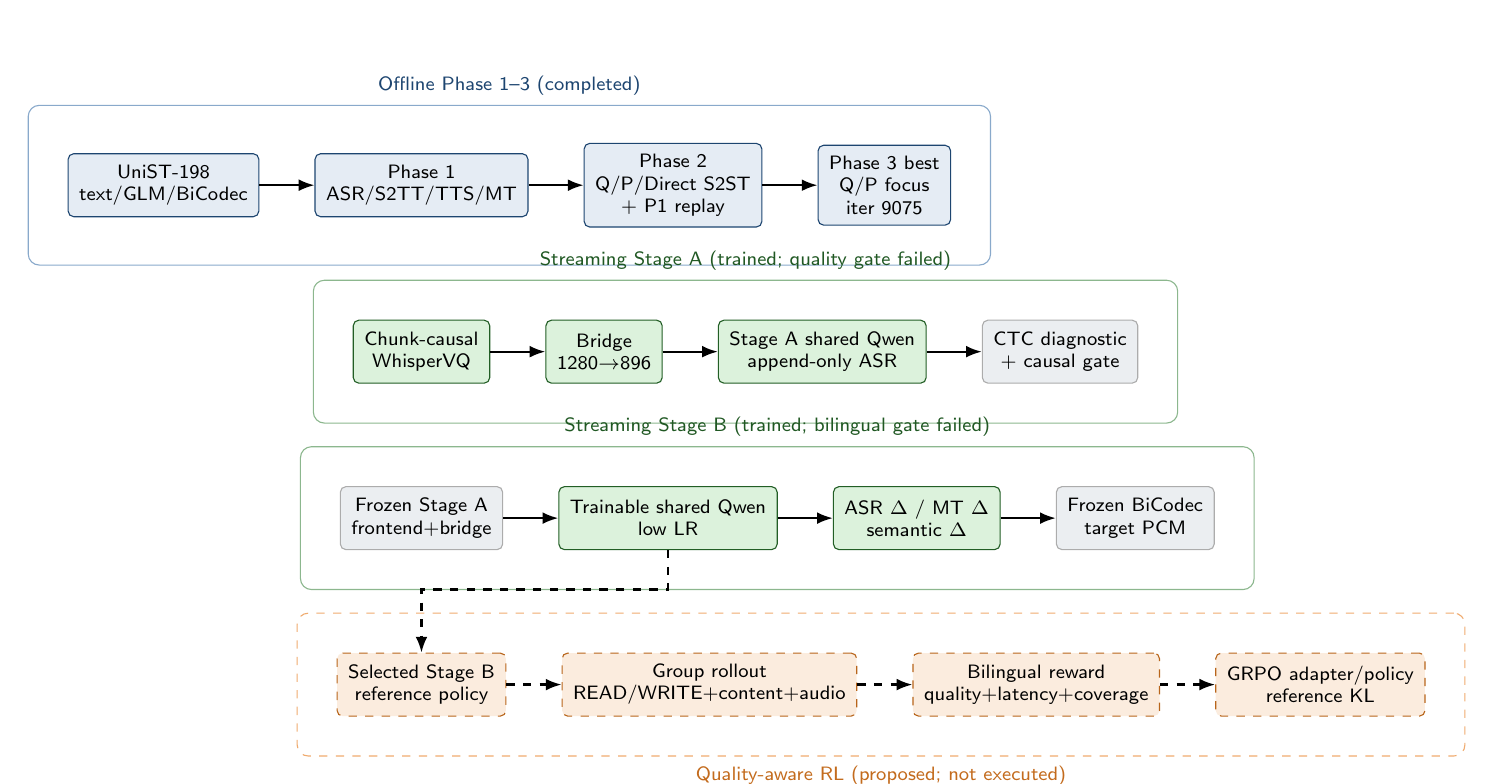
\begin{tikzpicture}[
  font=\sffamily\scriptsize,
  node distance=5mm and 7mm,
  box/.style={draw,rounded corners=2pt,align=center,minimum height=8mm,inner sep=4pt},
  offline/.style={box,fill=offlineblue!12,draw=offlineblue!70!black},
  stream/.style={box,fill=trainable,draw=streamgreen!75!black},
  freeze/.style={box,fill=frozen,draw=gray!65},
  future/.style={box,fill=futureorange!15,draw=futureorange!80!black,dashed},
  arr/.style={-{Latex[length=2mm]},thick},
  soft/.style={-{Latex[length=2mm]},dashed,thick}
]
  \node[offline] (data) {UniST-198\\text/GLM/BiCodec};
  \node[offline,right=of data] (p1) {Phase 1\\ASR/S2TT/TTS/MT};
  \node[offline,right=of p1] (p2) {Phase 2\\Q/P/Direct S2ST\\+ P1 replay};
  \node[offline,right=of p2] (p3) {Phase 3 best\\Q/P focus\\iter 9075};
  \draw[arr] (data)--(p1);
  \draw[arr] (p1)--(p2);
  \draw[arr] (p2)--(p3);

  \node[stream,below=13mm of p1] (causal) {Chunk-causal\\WhisperVQ};
  \node[stream,right=of causal] (bridge) {Bridge\\1280$\rightarrow$896};
  \node[stream,right=of bridge] (stageaq) {Stage A shared Qwen\\append-only ASR};
  \node[freeze,right=of stageaq] (ctc) {CTC diagnostic\\+ causal gate};
  \draw[arr] (causal)--(bridge);
  \draw[arr] (bridge)--(stageaq);
  \draw[arr] (stageaq)--(ctc);

  \node[freeze,below=13mm of causal] (fa) {Frozen Stage A\\frontend+bridge};
  \node[stream,right=of fa] (qwen) {Trainable shared Qwen\\low LR};
  \node[stream,right=of qwen] (deltas) {ASR $\Delta$ / MT $\Delta$\\semantic $\Delta$};
  \node[freeze,right=of deltas] (codec) {Frozen BiCodec\\target PCM};
  \draw[arr] (fa)--(qwen);
  \draw[arr] (qwen)--(deltas);
  \draw[arr] (deltas)--(codec);

  \node[future,below=13mm of fa] (rlinit) {Selected Stage B\\reference policy};
  \node[future,right=of rlinit] (rollout) {Group rollout\\READ/WRITE+content+audio};
  \node[future,right=of rollout] (reward) {Bilingual reward\\quality+latency+coverage};
  \node[future,right=of reward] (grpo) {GRPO adapter/policy\\reference KL};
  \draw[arr,dashed] (rlinit)--(rollout);
  \draw[arr,dashed] (rollout)--(reward);
  \draw[arr,dashed] (reward)--(grpo);
  \draw[soft] (qwen.south)--++(0,-5mm)-|(rlinit.north);

  \begin{scope}[on background layer]
    \node[draw=offlineblue!55,rounded corners,fit=(data)(p3),inner sep=5mm,label={[offlineblue!70!black]above:Offline Phase 1--3 (completed)}] {};
    \node[draw=streamgreen!55,rounded corners,fit=(causal)(ctc),inner sep=5mm,label={[streamgreen!70!black]above:Streaming Stage A (trained; quality gate failed)}] {};
    \node[draw=streamgreen!55,rounded corners,fit=(fa)(codec),inner sep=5mm,label={[streamgreen!70!black]above:Streaming Stage B (trained; bilingual gate failed)}] {};
    \node[draw=futureorange!65,rounded corners,dashed,fit=(rlinit)(grpo),inner sep=5mm,label={[futureorange!85!black]below:Quality-aware RL (proposed; not executed)}] {};
  \end{scope}
\end{tikzpicture}
}
  \caption{The complete UniSS offline--streaming--RL system. Stage A is initialized from the best Phase 3 checkpoint. Stage B freezes the causal acoustic frontend and updates the shared Qwen. Quality-aware RL is proposed only after the supervised quality gates are repaired.}
  \label{fig:architecture}
\end{figure*}

\section{Methodology}

\subsection{Offline Phase 1: Foundational Multitask Alignment}

Phase 1 first establishes the elementary mappings required by unified S2ST: source speech to transcription, source speech to translation, text plus speaker condition to target semantics, and transcription to translation as an MT proxy. Let the corresponding scalar losses be $\Loss_{\mathrm{asr}}$, $\Loss_{\mathrm{s2tt}}$, $\Loss_{\mathrm{tts}}$, and $\Loss_{\mathrm{mt}}$, each instantiated from \cref{eq:ce} with a different mask. If $\vect{\pi}^{(1)}\in[0,1]^4$ is the four-dimensional task-probability vector with $\sum_{j=1}^{4}\pi_j^{(1)}=1$, then
\begin{equation}
 \Loss_{\mathrm{P1}}
 =\E_{q\sim\mathrm{Cat}(\vect{\pi}^{(1)})}
 \left[\Loss_q\right].
 \label{eq:p1}
\end{equation}
The initial high-learning-rate run became unstable late in training. We therefore retained its 3,300-update checkpoint and performed 15,465 recovery updates with a lower learning rate, a fresh optimizer, and cyclic shuffle.

\subsection{Offline Phase 2: Direct S2ST with Capability Replay}

Phase 2 introduces Quality, Performance, and Direct S2ST examples. Its purpose is to learn the complete text-to-speech output path without overwriting the ASR, S2TT, TTS, and MT capabilities obtained in Phase 1. Let $\mathcal{D}_{\mathrm{P2}}$ and $\mathcal{D}_{\mathrm{P1}}$ denote the Phase 2 and replay distributions. The 2:1 mixture is
\begin{equation}
 \Loss_{\mathrm{P2}}
 =\frac{2}{3}\E_{u\sim\mathcal{D}_{\mathrm{P2}}}\Loss_{\mathrm{CE}}(u)
 +\frac{1}{3}\E_{v\sim\mathcal{D}_{\mathrm{P1}}}\Loss_{\mathrm{CE}}(v).
 \label{eq:p2}
\end{equation}
Phase 2 loads only the Phase 1 model weights, not its optimizer or random-number-generator state, which makes this handoff an independently auditable stage.

\subsection{Offline Phase 3: Quality/Performance Specialization}

Phase 3 starts from Phase 2 checkpoint `iter\_0015381` and retains only the final Quality and Performance tasks. Let $\mathcal{D}_Q$ and $\mathcal{D}_P$ denote the two distributions and let $\rho\in[0,1]$ be the Quality sampling probability. Then
\begin{equation}
 \Loss_{\mathrm{P3}}
 =\rho\,\E_{u\sim\mathcal{D}_{Q}}\Loss_{\mathrm{CE}}(u)
 +(1-\rho)\,\E_{v\sim\mathcal{D}_{P}}\Loss_{\mathrm{CE}}(v).
 \label{eq:p3}
\end{equation}
The Quality path generally emits an explicit source transcription, target translation, and target semantic sequence. The Performance path is shorter and balances output quality with generation length. Phase 3 changes the task distribution rather than adding a new network module.

\subsection{Streaming Stage A: Causal Acoustic Frontend and Incremental ASR}

Phase 3 consumes a complete source GLM sequence and cannot directly accept incrementally arriving PCM. Stage A converts a waveform prefix into an 80-dimensional log-Mel matrix $\mat{X}_{1:t}\in\R^{t\times80}$, where $t$ is the number of currently visible acoustic frames. The chunk-causal WhisperVQ encoder produces $\mat{A}_{1:u}=g_\phi(\mat{X}_{1:t},\mat{C}_{k-1})\in\R^{u\times1280}$, where $u$ is the visible encoded length and $\mat{C}_{k-1}$ is a cache containing only states from earlier chunks. The bridge maps the acoustic representation into the Qwen hidden dimension:
\begin{equation}
 \mat{E}^{\mathrm{ac}}=\operatorname{LN}(\mat{A})\mat{W}_{b}+\vect{b}_{b},
 \quad \mat{W}_{b}\in\R^{1280\times896},
 \quad \vect{b}_{b}\in\R^{896},
 \label{eq:bridge}
\end{equation}
yielding $\mat{E}^{\mathrm{ac}}\in\R^{u\times896}$ for injection into Qwen.

The declared Stage A objective is
\begin{align}
 \Loss_A={}&1.00\Loss_{\mathrm{AR\text{-}ASR}}
 +0.30\Loss_{\mathrm{CTC}}
 +0.20\Loss_{\mathrm{teacher\text{-}KL}}
 +0.10\Loss_{\mathrm{multi\text{-}chunk}}\nonumber\\
 &+0.10\Loss_{\mathrm{cache/full}}
 +1.00\Loss_{\mathrm{offline\text{-}ASR\text{-}replay}}
 +1.00\Loss_{\mathrm{P3\text{-}replay}}.
 \label{eq:stagea}
\end{align}
$\Loss_{\mathrm{AR\text{-}ASR}}$ is the append-only ASR-delta CE. For a source label sequence $\vect{a}\in\Vocab^J$ of length $J$ and a CTC posterior matrix $\mat{P}\in[0,1]^{u\times(V_{\mathrm{asr}}+1)}$, where $V_{\mathrm{asr}}$ is the ASR label-vocabulary size, CTC marginalizes all $u$-step blank-augmented paths:
\begin{equation}
 \Loss_{\mathrm{CTC}}=-\log\sum_{\vect{\pi}\in\mathcal{B}^{-1}(\vect{a})}
 \prod_{r=1}^{u}P_{r,\pi_r}.
 \label{eq:ctc}
\end{equation}
Here $\vect{\pi}$ is a length-$u$ alignment path and $\mathcal{B}$ removes blanks and repeated labels. The multi-chunk term encourages compatible representations for the same audio at different chunks, while the replay terms preserve offline capabilities. Importantly, the formal run had a zero effective denominator for teacher KL, and cache/full consistency was implemented as an external gate. Neither term can therefore be credited with an observed gain.

The decision-chunk curriculum is defined by coverage progress $r\in[0,1]$:
\begin{equation}
 \mathcal{C}(r)=
 \begin{cases}
 \{1280,960\}\ \mathrm{ms}, & 0\le r<0.10,\\
 \{960,640\}\ \mathrm{ms}, & 0.10\le r<0.35,\\
 \{640,320\}\ \mathrm{ms}, & 0.35\le r<0.70,\\
 \{320,160\}\ \mathrm{ms}, & 0.70\le r\le1.
 \end{cases}
 \label{eq:chunkcurr}
\end{equation}

\subsection{Streaming Stage B: Five-Family Joint Incremental Training}

Stage A builds a streaming ASR interface but does not ensure incremental translation or continuous target speech. Stage B therefore freezes WhisperVQ, the bridge, and the CTC head, and updates only the shared Qwen. The maximum learning rates are $2\times10^{-6}$ for the Transformer body and $5\times10^{-7}$ for the tied embedding/LM head.

Each utterance is converted into a trajectory $\vect{\tau}=(e_1,\ldots,e_K)$ of $K$ events. Event $k$ is
\begin{equation}
 e_k=(t_k,\Delta\vect{a}_k,\Delta\vect{b}_k,
 \Delta\vect{u}_k,q_k),
 \label{eq:event}
\end{equation}
where $t_k\in\R_{\ge0}$ is the source time, $\Delta\vect{a}_k\in\Vocab^{J_k}$ is the ASR increment, $\Delta\vect{b}_k\in\Vocab^{M_k}$ is the target-text increment, $\Delta\vect{u}_k\in\Vocab^{U_k}$ is the target-semantic increment, and $q_k\in[0,1]$ is alignment confidence. $J_k$, $M_k$, and $U_k$ are the three increment lengths. Gold histories provide stable supervision, while free-running histories expose the model to its own prefix errors. Records are routed into clean, noisy-content, and quarantine strata. Quarantined examples may participate in Phase 3 replay but not in the strict incremental tasks.

The steady task mixture is 25\% streaming ASR, 20\% incremental MT, 30\% end-to-end S2ST, 15\% Phase 3 Quality replay, and 10\% Phase 3 Performance replay. The active objective is
\begin{align}
 \Loss_B={}&1.00\Loss_{\mathrm{ASR}-\Delta}
 +1.00\Loss_{\mathrm{MT}-\Delta}
 +1.00\Loss_{\mathrm{semantic}-\Delta}
 +0.50\Loss_{\mathrm{replay}}\nonumber\\
 &+0.30\Loss_{\mathrm{V1\text{-}ASR\text{-}KL}}
 +0.25\Loss_{\mathrm{P3\text{-}KL}}
 +0.20\Loss_{\mathrm{commit}}
 +0.10\Loss_{\mathrm{boundary}}\nonumber\\
 &+0.50\Loss_{\mathrm{semantic\text{-}END}}
 +0.25\Loss_{\mathrm{END\text{-}margin}}.
 \label{eq:stageb}
\end{align}
For two events sharing a committed prefix, let the student posteriors at protected position $i$ be $\vect{p}^{(k)}_i,\vect{p}^{(k+1)}_i\in[0,1]^{V'}$. For the protected-position set $\mathcal{I}$, the commit-consistency loss is
\begin{equation}
 \Loss_{\mathrm{commit}}=
 \frac{1}{|\mathcal{I}|}\sum_{i\in\mathcal{I}}
 \KL\!\left(\vect{p}^{(k)}_i\middle\|\vect{p}^{(k+1)}_i\right).
 \label{eq:commitkl}
\end{equation}
To discourage a premature semantic END, let $l_{\mathrm{end}}\in\R$ be its logit, $l_y\in\R$ the logit of the correct content token, and $m=2$ the scalar margin. Then
\begin{equation}
 \Loss_{\mathrm{END\text{-}margin}}
 =\max\left(0,m+l_{\mathrm{end}}-l_y\right).
 \label{eq:endmargin}
\end{equation}
The loss prefers $l_y\ge l_{\mathrm{end}}+m$ before the content is complete. It does not determine whether the upstream prefix is correct; consequently, it may also prolong an incorrect translation after an irreversible ASR error.

\subsection{Proposed RL Stage: Quality-Aware Trajectory-Level GRPO}

The previous GRPO route froze the backbone and trained only a binary action head. Such a policy cannot directly repair translation content or semantic completeness. The proposed RL stage starts from Stage B `iter\_0001132`, or from a later quality-repaired selected checkpoint. The acoustic frontend and BiCodec remain frozen. A top-layer Qwen adapter and action policy are trainable, while content and semantic posteriors are protected with strong reference KL.

For input $\vect{s}$, sample $G$ complete trajectories $\{\vect{\tau}_i\}_{i=1}^{G}$. Define
\begin{align}
 R_i={}&w_q Q_i+w_p P_i-w_f\widetilde{F}_i-w_a\widetilde{A}_i
 -w_l\widetilde{L}_i-w_{\mathrm{pre}}U_i-w_{\mathrm{wait}}W_i\nonumber\\
 &+w_c C_i+w_s S_i+w_b B_i,
 \label{eq:reward}
\end{align}
where $Q_i,P_i,C_i,S_i,B_i\in[0,1]$ are normalized bilingual final quality, prefix support, completeness, semantic non-silence, and boundary continuity. $\widetilde{F}_i,\widetilde{A}_i,\widetilde{L}_i\in\R_{\ge0}$ are normalized First WRITE, ATD, and LAAL; $U_i,W_i\in[0,1]$ are premature WRITE and unnecessary WAIT. All scalar weights $w_\cdot\ge0$.

The group reward statistics are
\begin{equation}
 \mu_R=\frac1G\sum_{i=1}^G R_i,
 \qquad
 \sigma_R=\sqrt{\frac1G\sum_{i=1}^G(R_i-\mu_R)^2},
 \label{eq:groupstats}
\end{equation}
and the normalized scalar advantage is
\begin{equation}
 A_i=\frac{R_i-\mu_R}{\sigma_R+\epsilon},
 \label{eq:advantage}
\end{equation}
where $\epsilon>0$ prevents division by zero. With trainable policy $\pi_\theta$, frozen reference policy $\pi_{\mathrm{ref}}$, KL weight $\beta\ge0$, and replay weight $\lambda_{\mathrm{replay}}\ge0$, the objective is
\begin{equation}
 \Loss_{\mathrm{GRPO}}
 =-\frac1G\sum_{i=1}^{G}A_i\log\pi_\theta(\vect{\tau}_i\mid\vect{s})
 +\beta\KL\!\left(\pi_\theta\middle\|\pi_{\mathrm{ref}}\right)
 +\lambda_{\mathrm{replay}}\Loss_{\mathrm{replay}}.
 \label{eq:grpo}
\end{equation}
An RL gain will be accepted only if it outperforms matched continued SFT in both quality retention and latency, and if at least one operating point lies above and to the left of the fixed wait-$k$ quality--latency frontier.

\section{Experiments}

\subsection{Dataset Composition}

The principal dataset is public UniST. The training set contains 198 parquet shards and 19,785,924 records; dev contains 7,965 records and test contains 23,369. Each record provides an ID, source and target language, source transcription, target translation, source GLM tokens, source and target BiCodec semantic tokens, and 32 global speaker tokens. Offline sample and packing counts are given in \cref{tab:data_scale}.

\begin{table}[H]
\centering
\caption{Offline Phase 1--3 data scale. The Phase 2 ratio denotes new-task examples to Phase 1 replay.}
\label{tab:data_scale}
\begin{tabularx}{\textwidth}{lrrY}
\toprule
Stage & Unpacked samples & 18k packed samples & Task composition \\
\midrule
Phase 1 & 79,143,696 & 800,632 & ASR, S2TT, TTS, and MT proxy \\
Phase 2 raw & 59,357,772 & \multirow{2}{*}{1,968,716} & Quality, Performance, and Direct S2ST \\
Phase 2 + replay & 89,036,658 & & Phase 2:Phase 1 replay = 2:1 \\
Phase 3 & 39,571,848 & 1,161,587 & Quality and Performance \\
\bottomrule
\end{tabularx}
\end{table}

Streaming Stage A/B uses a fixed 15-shard pilot for controlled iteration. Stage A includes 1,325,243 source records and 16,195 packed training sequences. Stage B expands the same utterances into 25,997,984 training events and 263,391 validation events. Of the training events, 7,666,418 contain a non-empty target WRITE before source EOS. Quality routing produces 385,051 clean, 616,445 noisy-content, and 323,747 quarantine records.

\paragraph{Discussion.}
The full198 offline data provides broad capability coverage, whereas the fixed 15-shard streaming pilot enables faster causal iteration and matched comparisons. Conclusions about the streaming stages are therefore pilot conclusions, not full-corpus generalization claims.

\subsection{Data Construction and a Real Example}

Offline preparation maps each parquet record into task-conditioned JSONL and then packs multiple examples into sequences of length 18,000 with reset attention masks. Stage B additionally stores event time, ASR/MT/semantic deltas, alignment confidence, gold/free-running history, and the quality route.

The first record of `train-00000.parquet` is a real English-to-Chinese example:
\begin{lstlisting}
id: NCSSD_R_EN_0000000000
src_lang: eng
tgt_lang: cmn
transcription:
  Hello, I'm looking for a book on mindfulness. Can you help me?
translation (verbatim):
  你好，我在寻找一本关于正念的书。你能帮我吗？
English gloss:
  Hello, I am looking for a book on mindfulness. Can you help me?
source_glm length: 53
source_bicodec length: 211
target_bicodec length: 178
bicodec_global length: 32
\end{lstlisting}
The Chinese reference is stored verbatim in the data; the English gloss above is used only to keep this report fully English. Stage B converts this utterance into 15 streaming events. The first four are summarized in \cref{tab:event_demo}.

\begin{table}[H]
\centering
\caption{Stage B trajectory demo constructed from one real UniST record.}
\label{tab:event_demo}
\small
\begin{tabularx}{\textwidth}{crrYYYc}
\toprule
Event & Start/ms & End/ms & Source delta/prefix & Target delta & Semantic slice & Confidence \\
\midrule
0 & 0 & 480 & `Hello' & empty & empty & -- \\
1 & 480 & 640 & prefix=`Hello' & `你好' & $[0{:}28]$ & 0.7227 \\
2 & 640 & 800 & `I'm' & empty & empty & -- \\
3 & 800 & 960 & updated source prefix & `我在' & $[28{:}40]$ & 0.6443 \\
\bottomrule
\end{tabularx}
\end{table}

\paragraph{Discussion.}
An empty target delta means that the visible source prefix does not yet support a safe translation commit; it is not a missing label. Confidence values near 0.64--0.72 also demonstrate why automatically generated trajectories cannot be treated as perfect ground truth. Quality routing is essential before irreversible supervision is applied.

\subsection{Model and Training Configuration}

The offline backbone is a 24-layer Qwen2.5-0.5B model with hidden size 896, FFN size 4,864, 14 attention heads, 2 KV heads, sequence length 18,000, and BF16 precision. Megatron-LM runs on one 8-GPU node with tensor parallelism 1, pipeline parallelism 1, micro batch 2, global batch 128, AdamW with $(\beta_1,\beta_2)=(0.9,0.95)$, and FlashAttention.

\begin{table}[H]
\centering
\caption{Training budgets and representative final validation losses. Stage B validation is a post-training fixed-16 free-running gate, not an in-loop held-out loss.}
\label{tab:training_budget}
\small
\begin{tabularx}{\textwidth}{lr>{\raggedright\arraybackslash}p{0.16\textwidth}>{\raggedright\arraybackslash}p{0.17\textwidth}Y}
\toprule
Stage & Updates & Data scope & Representative loss & Initialization / trainable scope \\
\midrule
Phase 1 & 3,300 + 15,465 & UniST-198 & approximately 5.3098 & Full model; low-LR recovery \\
Phase 2 & 15,381 & UniST-198 & approximately 4.2881 & Full model from Phase 1 \\
Phase 3 & 9,075 & UniST-198 & 3.80985 & Full model from Phase 2 \\
Stage A & 381 & 15 shards; 3 coverages & numerically stable & Causal frontend, bridge, and shared Qwen \\
Stage B & 2,264 & 15 shards; 3 coverages & multitask trade-off & Frozen frontend; shared Qwen only \\
\bottomrule
\end{tabularx}
\end{table}

\paragraph{Discussion.}
The offline runs optimize all model parameters, whereas Stage B deliberately freezes the causal frontend and uses much smaller learning rates for Qwen. This separation improves attribution but does not guarantee ASR retention because the shared decoder posterior still changes.

\subsection{Evaluation Metrics}

Text quality is measured with corpus Text-BLEU. Speech-BLEU first transcribes generated target speech with a target-language ASR system and then computes BLEU, so it includes translation, synthesis, and evaluation-ASR errors. AutoPCP is an automatic proxy for cross-lingual prosody/expression similarity. UTMOS estimates perceptual naturalness. For source and generated durations $d_s,d_y\in\R_{>0}$ and $M$ evaluated examples, duration consistency is
\begin{equation}
 \mathrm{SLC}_{\delta}
 =\frac1M\sum_{i=1}^{M}
 \mathbb{I}\left(1-\delta\le\frac{d_y^{(i)}}{d_s^{(i)}}\le1+\delta\right),
 \label{eq:slc}
\end{equation}
where $\delta\in\{0.2,0.4\}$ and $\mathrm{SLC}_{\delta}\in[0,1]$.

Streaming ASR uses WER or CER. First WRITE and First audio are the consumed source times at the first non-empty target-text commit and first playable non-silent target waveform. If target token $j$ is written at source time $g(j)\in\R_{\ge0}$, the generated target length is $L$, the reference length is $L^*$, and source duration is $d_s$, the current diagnostic average-token-delay proxy is
\begin{equation}
 \mathrm{ATD}_{\mathrm{proxy}}
 =\frac{1}{L}\sum_{j=1}^{L}\left[g(j)-\frac{j-1}{\max(L^*,1)}d_s\right].
 \label{eq:atdproxy}
\end{equation}
The diagnostic utterances do not have strict human word- or audio-level alignments; therefore reported LAAL and ATD values are explicitly proxies and are not directly comparable to standardized SimulEval values. Runtime factor is $\mathrm{RTF}=t_{\mathrm{wall}}/d_s$. Batch-one RTF below 1 means computation is faster than real time, not that the policy emits early.

\paragraph{Discussion.}
No single metric is sufficient. A lower First audio may indicate a useful early translation, an incomplete output, or an early error. Every latency result must therefore be paired with content, completeness, non-silence, and final-flush measurements.

\section{Experimental Results and Discussion}

\subsection{Offline Phase 1--3: Convergence and Curriculum Gain}

Validation loss decreases from approximately 5.31 after Phase 1 recovery to 4.29 after Phase 2 and 3.81 after Phase 3. The Phase 1 recovery removes late high-LR instability. Phase 2 adds direct S2ST with replay, and Phase 3 specializes the task distribution.

\begin{table}[H]
\centering
\caption{Aggregate Phase 2-to-Phase 3 changes on UniST dev/test under the same protocol.}
\label{tab:p2p3_summary}
\begin{tabularx}{\textwidth}{lCCY}
\toprule
Split & Improved cells & Degraded cells & Interpretation \\
\midrule
dev & 23/24 & 1/24 & Broad improvements in AutoPCP, SLC, and BLEU \\
test & 21/24 & 3/24 & Translation and semantic metrics improve; limited decreases concentrate in UTMOS \\
\bottomrule
\end{tabularx}
\end{table}

\paragraph{Discussion.}
The improvement is attributable to curriculum and task concentration rather than a new architecture. The 21/24 test result supports the ordering ``broad alignment, direct S2ST with replay, final-task specialization.'' The remaining UTMOS decreases show that token-level CE does not perfectly represent perceptual naturalness.

\subsection{Offline Phase 3: Best UniST Test Results}

\begin{table}[H]
\centering
\caption{Best Offline Phase 3 checkpoint `iter\_0009075` on UniST test.}
\label{tab:p3_test}
\resizebox{\textwidth}{!}{%
\begin{tabular}{llrrrrrr}
\toprule
Mode & Direction & Text-BLEU & Speech-BLEU & AutoPCP & SLC-0.2 & SLC-0.4 & UTMOS \\
\midrule
Performance & ZH$\rightarrow$EN & 32.4509 & 19.3770 & \textbf{2.9118} & 0.6324 & \textbf{0.8782} & 3.6676 \\
Performance & EN$\rightarrow$ZH & 40.5404 & 38.9953 & \textbf{3.2765} & 0.7184 & \textbf{0.9421} & 3.3516 \\
Quality & ZH$\rightarrow$EN & \textbf{39.3753} & \textbf{22.7268} & 2.8850 & \textbf{0.6358} & 0.8712 & \textbf{3.6680} \\
Quality & EN$\rightarrow$ZH & \textbf{48.1698} & \textbf{46.3063} & 3.2752 & \textbf{0.7246} & 0.9349 & \textbf{3.3586} \\
\bottomrule
\end{tabular}}
\end{table}

\paragraph{Discussion.}
Quality mode produces higher Text- and Speech-BLEU in both directions, supporting the value of explicit intermediate text. Performance mode is nevertheless competitive or better on some AutoPCP/SLC cells, showing that a shorter generation path does not uniformly degrade all speech attributes. ZH-to-EN Speech-BLEU remains substantially lower than EN-to-ZH, making English target-speech intelligibility and semantic generalization a primary offline weakness.

\subsection{Streaming Stage A: A Working Causal Interface with a Failed Free-Running Gate}

Stage A finishes all 381 updates with zero skipped iterations and zero NaNs. It generates pre-final output for 972/972 events, demonstrating that the causal visibility path and event grammar execute correctly. Free-running ASR, however, remains far from the offline anchor.

\begin{table}[H]
\centering
\caption{Stage A formal training and free-running ASR results.}
\label{tab:stagea}
\begin{tabularx}{\textwidth}{lrrY}
\toprule
Metric & Stage A & Offline anchor & Interpretation \\
\midrule
Weighted WER/CER & 27.1432\% & -- & Bilingual aggregate; gate failed \\
Chinese CER & 21.0112\% & 5.4661\% & Large causal-chunk degradation \\
English WER & 35.3399\% & 5.6072\% & More severe English degradation \\
Causal-full error & 14.4546\% & -- & Complete causal input is easier than chunked free-running \\
Teacher-forced accuracy & 92.0737\% & -- & Strong prediction under correct history \\
CTC all-blank cases & 15 & 0 expected & CTC supplies no valid alignment for some samples \\
Event-stop failures & 27 & 0 expected & Structural stopping failures remain \\
\bottomrule
\end{tabularx}
\end{table}

\paragraph{Discussion.}
The gap between 92.07\% teacher-forced accuracy and 27.14\% free-running error indicates exposure-bias and irreversible-prefix accumulation rather than a complete inability to predict ASR tokens. The causal-full result of 14.45\% further isolates an additional chunk-boundary/state-propagation penalty. Stage A is therefore a structurally successful but quality-gate-failed causal checkpoint.

\subsection{Streaming Stage B: Learned Objectives and Multitask Conflict}

Stage B completes three 15-shard coverage epochs and 2,264 updates with no skipped iterations or NaNs. ASR CE, MT CE, and semantic END margin decrease, but replay, KL retention, and boundary objectives do not improve together.

\begin{table}[H]
\centering
\caption{Means over the first and last 10\% of non-zero Stage B training scalars.}
\label{tab:stageb_losses}
\begin{tabularx}{\textwidth}{llrrY}
\toprule
Segment & Metric & Early & Late & Trend \\
\midrule
Epoch 1 & ASR CE & 1.716 & 0.954 & improved \\
Epoch 1 & MT CE & 4.699 & 2.079 & improved \\
Epoch 1 & semantic END margin & 2.528 & 0.070 & strongly improved \\
Epoch 1 & replay CE & 4.018 & 4.056 & flat/slightly worse \\
Epoch 1 & V1 ASR KL & 0.255 & 0.338 & retention drift increased \\
Epoch 2--3 & ASR CE & 0.818 & 0.684 & improved \\
Epoch 2--3 & MT CE & 2.098 & 1.780 & improved \\
Epoch 2--3 & semantic END margin & 0.070 & 0.046 & improved \\
Epoch 2--3 & boundary/EOS & 0.198 & 0.534 & degraded \\
Epoch 2--3 & content END CE & 0.830 & 1.096 & degraded \\
\bottomrule
\end{tabularx}
\end{table}

\paragraph{Discussion.}
The END-margin objective is clearly learnable, but boundary/EOS and content-END losses move in the opposite direction. V1 ASR KL also rises, showing that freezing the acoustic frontend does not freeze the streaming ASR behavior of the shared decoder. A future supervised revision should adapt retention weights using bilingual free-running gates rather than further increasing END-margin alone.

\subsection{Streaming Stage B: Checkpoint Selection and Directional Asymmetry}

\begin{table}[H]
\centering
\caption{Fixed-16 free-running validation for three Stage B checkpoints. Lower ASR error and higher chrF/coverage are better.}
\label{tab:stageb_ckpt}
\resizebox{\textwidth}{!}{%
\begin{tabular}{lrrrrrr}
\toprule
Checkpoint & Chinese ASR error & English ASR error & free ZH$\rightarrow$EN chrF & free EN$\rightarrow$ZH chrF & semantic coverage & non-silent \\
\midrule
iter 1132 & 0.1174 & 0.3097 & \textbf{24.078} & \textbf{5.414} & \textbf{0.875} & \textbf{7/8} \\
iter 1207 & 0.1033 & 0.3355 & 21.312 & 4.827 & 0.682 & 6/8 \\
iter 2264 & \textbf{0.0892} & \textbf{0.3032} & 21.216 & 4.630 & 0.797 & \textbf{7/8} \\
\bottomrule
\end{tabular}}
\end{table}

\paragraph{Discussion.}
The final checkpoint has the best ASR retention, but iter 1132 has the best free-running MT and semantic coverage. Continued training therefore improves local ASR while reducing translation quality. All three checkpoints fail the combined structure, coverage, and non-silence gates. Iter 1132 is only the best diagnostic listening candidate among failed checkpoints, not a formally selected model.

\subsection{Matched Stage A/B Audio: Latency and Content}

The strict causal cascade consumes physical PCM in 160\,ms blocks and makes decisions at 160, 320, 640, or 1,280\,ms intervals. MT reads only committed ASR, and TTS reads only newly committed target text. \Cref{tab:en2zh_latency} reports a 4.22-s English-to-Chinese utterance.

\begin{table}[H]
\centering
\caption{English-to-Chinese Stage A/B First audio and content. Times are in ms; LAAL is a proxy.}
\label{tab:en2zh_latency}
\resizebox{\textwidth}{!}{%
\begin{tabular}{lrrrrrl}
\toprule
Stage & Chunk & First ASR & First MT & First audio & LAAL proxy & Generated translation \\
\midrule
A & 160 & 1120 & 1600 & 4220 & 1378 & `Hello, I' equivalent \\
B & 160 & \textbf{960} & 1600 & \textbf{2400} & 1793 & More content, but incomplete \\
A & 320 & 1280 & 1920 & 4220 & 1698 & `Hello, I' equivalent \\
B & 320 & 1280 & 1920 & \textbf{2880} & 2033 & More content, but incomplete \\
A & 640 & 1920 & 3200 & 4220 & 2105 & Complete and correct \\
B & 640 & 1920 & \textbf{2560} & 4220 & \textbf{1885} & Complete and correct \\
A & 1280 & 2560 & 4220 & 4220 & 2332 & Complete and correct \\
B & 1280 & 2560 & \textbf{3840} & 4220 & \textbf{2181} & Complete and correct \\
\bottomrule
\end{tabular}}
\end{table}

The short-chunk First-audio improvements are
\begin{equation}
 \Delta F_{160}=4220-2400=1820\ \mathrm{ms},\qquad
 \Delta F_{320}=4220-2880=1340\ \mathrm{ms}.
 \label{eq:firstaudio_gain}
\end{equation}
These are the clearest latency gains produced by the current streaming innovation, but the corresponding outputs are incomplete. At 640/1280\,ms, content is retained while First audio remains at source EOS.

\begin{table}[H]
\centering
\caption{Chinese-to-English Stage A/B First audio and generated content for a 9.66-s source.}
\label{tab:zh2en_latency}
\resizebox{\textwidth}{!}{%
\begin{tabular}{lrrrrl}
\toprule
Stage & Chunk & First ASR & First MT & First audio & Generated translation \\
\midrule
A & 160 & 960 & 1760 & 2560 & `That actually,' incomplete \\
B & 160 & 1120 & 1440 & 1760 & `The horse actually waited for us,' incorrect \\
A & 320 & 1280 & 2240 & 9660 & `That,' incomplete \\
B & 320 & 1280 & 1920 & 2240 & `The horse ...,' incorrect \\
A & 640 & 1920 & 4480 & 6400 & Complete and semantically reasonable \\
B & 640 & 1920 & 2560 & 3840 & `The horse actually waited for us,' incorrect \\
A & 1280 & 2560 & 6400 & 7680 & Complete and semantically reasonable \\
B & 1280 & 2560 & 3840 & 9660 & `The,' truncated \\
\bottomrule
\end{tabular}}
\end{table}

\paragraph{Discussion.}
The lower Chinese-to-English First audio of Stage B is caused by an incorrect irreversible ASR prefix, which is translated as ``The horse.'' It is not a valid latency improvement. This result demonstrates why simultaneous metrics must be accompanied by semantic correctness and completeness: an early or negative end offset may simply mean that the model speaks incorrectly or stops too soon.

\subsection{Earlier Action-Only GRPO: Better Quality but No Latency Gain}

The earlier Stage7A comparison evaluates a Stage6 baseline (E0), matched continued SFT (E1), GRPO with group size 4 (E2), and GRPO with group size 8 (E3) on 23,369 test examples. The backbone is frozen and only a WAIT/WRITE action head is trained.

\begin{table}[H]
\centering
\caption{Main quality and latency results of the earlier action-only GRPO experiment. This is not RL on the current Stage B model.}
\label{tab:old_grpo}
\resizebox{\textwidth}{!}{%
\begin{tabular}{lrrrrrr}
\toprule
Experiment & Text-BLEU ZH$\rightarrow$EN & Text-BLEU EN$\rightarrow$ZH & First WRITE & ATD & Premature & Unnecessary WAIT \\
\midrule
E0 Stage6 & 26.378 & \textbf{40.560} & \textbf{3986.4} & \textbf{1807.3} & 0.031 & 0.158 \\
E1 continued SFT & 26.240 & 40.480 & 3991.0 & 1808.4 & 0.030 & 0.157 \\
E2 GRPO G4 & 27.587 & 40.224 & 4055.4 & 1839.0 & \textbf{0.027} & 0.164 \\
E3 GRPO G8 & \textbf{28.109} & 40.355 & 4032.8 & 1827.5 & 0.029 & 0.162 \\
\bottomrule
\end{tabular}}
\end{table}

Relative to matched E1, E3 improves ZH-to-EN Text-BLEU by $28.109-26.240=1.869$ but increases First WRITE by 41.85\,ms and ATD by 19.14\,ms. GRPO reduces a small amount of premature WRITE while increasing unnecessary WAIT.

\paragraph{Discussion.}
This experiment is a direct counterexample to the claim that adding RL necessarily reduces latency. Without explicit First WRITE/ATD, bilingual quality, completeness, and audio-validity terms, the group-relative objective prefers safer but slower trajectories. This failure motivates the multi-component reward in \cref{eq:reward}.

\subsection{Reward-v2 Evidence and the Acceptance Criteria for Future RL}

Reward-v2 experiments R0--R3 add coverage, explicit latency, and bilingual/adaptive-KL terms on the older Stage6 action-head route. They are preliminary evidence and must not be attributed to Stage B.

\begin{table}[H]
\centering
\caption{Reward-v2 dev results. R1 is the matched rebalanced-plus-coverage control.}
\label{tab:rewardv2}
\resizebox{\textwidth}{!}{%
\begin{tabular}{lrrrrrr}
\toprule
Experiment & ZH$\rightarrow$EN Text-BLEU & EN$\rightarrow$ZH Text-BLEU & First WRITE & ATD & Premature & Unnecessary WAIT \\
\midrule
R0 E3-v1+bias & 27.592 & 37.724 & 4205.6 & 1890.0 & 0.032 & 0.150 \\
R1 coverage & 28.952 & 37.610 & 4234.1 & 1907.9 & 0.031 & 0.149 \\
R2 explicit latency & 28.983 & 37.458 & \textbf{4111.2} & \textbf{1861.4} & 0.037 & \textbf{0.141} \\
R3 bilingual+adaptive KL & \textbf{29.277} & \textbf{37.694} & 4157.5 & 1883.2 & 0.035 & 0.144 \\
\bottomrule
\end{tabular}}
\end{table}

Relative to R1, R2 reduces First WRITE and ATD by 122.9/46.5\,ms while reducing EN-to-ZH Text-BLEU by 0.152. R3 reduces First WRITE and ATD by 76.6/24.7\,ms and improves the two Text-BLEU directions by 0.325/0.084.

\paragraph{Discussion.}
These trends support bilingual quality terms and adaptive KL, but they remain single-seed dev evidence. A future Stage B RL study must include matched continued SFT, the fixed wait-$k$ frontier, at least three seeds, 10,000 paired-bootstrap samples, batch-one latency, both Text- and Speech-BLEU directions, UTMOS/AutoPCP, premature/unnecessary WAIT, final flush, completeness, and non-silence.

\section{Ablation Interpretation and Error Analysis}

\subsection{Value and Limits of Replay}

The Phase 2 replay plus Phase 3 specialization pipeline improves 21 of 24 principal test cells, supporting replay as an effective offline curriculum mechanism. In Stage B, however, replay CE is nearly flat and V1 ASR KL increases. Fixed weights of 0.50 for replay and 0.30 for ASR KL are therefore insufficient to prevent posterior drift in the shared Qwen. Future retention weights should respond to bilingual free-running gates instead of only to training CE.

\subsection{Scope of the Chunk Curriculum}

Multi-chunk training allows one checkpoint to support 160--1,280\,ms operating points rather than requiring a separate model for each delay. Short chunks nevertheless contain less semantic evidence and are more likely to cause permanent prefix errors. The combination of earlier incomplete English-to-Chinese speech and early incorrect Chinese-to-English speech shows that chunk curriculum must be paired with prefix-support supervision.

\subsection{The Double-Edged Effect of END Margin}

Semantic END margin decreases from 2.528 to 0.070, proving that the objective is learnable, while boundary/EOS and content-END CE degrade later. END margin answers whether generation should continue, not whether the current content is correct. When ASR is wrong, a stronger margin can make the wrong semantic sequence longer and more confident. It should be gated by translation coverage, source-prefix support, and teacher posterior reliability.

\subsection{Speaker Consistency and Audio Continuity}

The Stage B speaker-continuity weight is zero because no reliable cross-fragment speaker-embedding sidecar is available. Offline Phase 3 conditions synthesis on 32 global BiCodec tokens from the source speaker. Keeping these tokens fixed helps preserve global identity, but fragmented semantic generation, short codec context, and incorrect language content can still change perceived timbre. Future work should add genuine cross-fragment speaker-embedding consistency and boundary cross-fade/holdback evaluation; AutoPCP alone is not proof of speaker identity.

\section{Limitations and Threats to Validity}

\begin{itemize}
  \item The offline results are a public UniST-198 reproduction with a 0.5B backbone, not an exact reproduction of the original UniSS 1.5B system and its complete corpus. The numbers must not be presented as a direct paper ranking.
  \item Stage A/B are trained on a fixed 15-shard pilot. Stage B selection uses a fixed-16 free-running gate, and the matched audio latency analysis contains only two representative utterances. These results do not establish population-level significance.
  \item Stage A teacher KL has a zero effective denominator, while cache/full consistency is an external gate. Neither can be claimed as an experimentally validated loss contribution.
  \item Stage B has no conventional in-loop held-out validation loss. Its validation values are post-training fixed-16 free-running gates.
  \item LAAL and ATD are proxy values derived from causal commit times without strict human source--target alignment. They cannot be directly ranked against standardized values reported by other papers.
  \item E0--E3 and R0--R3 use a frozen Stage6 action head and are not full content/semantic RL on Stage B. They are evidence for reward design only.
  \item Stage B's short-chunk English-to-Chinese First-audio gains are accompanied by incomplete content, while earlier Chinese-to-English output is incorrect. We claim a local first-packet improvement, not a bidirectional overall S2ST success.
\end{itemize}

\section{Conclusion and Next Steps}

This report provides a unified account of Offline Phase 1--3 and Streaming Stage A/B. The three-phase offline curriculum trains stably on the full public data and produces the current best checkpoint, Phase 3 `iter\_0009075`, which improves 21 of 24 principal UniST test cells over Phase 2. Stage A establishes a causal PCM-to-acoustic-embedding-to-append-only-ASR path but does not pass the free-running ASR gate. Stage B jointly trains incremental ASR, MT, semantics, and replay in the shared Qwen. It reduces English-to-Chinese First audio by 1.82/1.34\,s at 160/320\,ms chunks, but exposes severe directional asymmetry and irreversible-error propagation.

The next step should not be an immediate full-data expansion or a repetition of action-only GRPO. The recommended sequence is: (1) repair Chinese-to-English irreversible ASR/MT errors using stronger free-running retention and prefix-support objectives; (2) add a strict validation split, larger bidirectional causal evaluation, and non-proxy alignment; (3) apply the quality-aware GRPO objective in \cref{eq:reward,eq:grpo} to a genuinely selected Stage B checkpoint; and (4) expand to full198 only after bilingual quality, complete non-silent speech, and latency improve together. The central methodological contribution is not the concealment of failed gates, but the separation of offline quality, causal executability, and true Pareto improvement within one auditable model and data pipeline.

\appendix
\section{Reproducibility Assets}

\begin{longtable}{p{0.28\textwidth}p{0.66\textwidth}}
\toprule
Asset & Repository-relative path \\
\midrule
\endfirsthead
\toprule
Asset & Repository-relative path \\
\midrule
\endhead
Offline overview & \path{docs/uniss_training_reproduction/uniss_project_offline_phase1_3_and_streaming_stage_a_b_colleague_overview.md} \\
Phase 2/3 evaluation & \path{docs/uniss_training_reproduction/uniss_full198_phase2_phase3_detailed_evaluation_report.md} \\
Stage A result & \path{reports/uniss_phase3_v4_quality_first_true_streaming_pilot15_v1/stage_a_formal/stage_a_formal8_20260816T224100Z/STAGE_A_RESULT_REPORT.md} \\
Stage B implementation audit & \path{docs/uniss_training_reproduction/uniss_phase3_v4_e2e_simuls2st_native_megatron_implementation_report.md} \\
Stage A/B audio evaluation & \path{eval_outputs/uniss_phase3_v4_e2e_simuls2st_pilot15_v1/stage_b_endmargin_best_iter1132_stage_a_protocol_20260825T114500Z/STAGE_B_VS_STAGE_A_STREAMING_EVALUATION_REPORT.md} \\
Earlier GRPO test & \path{eval_outputs/simul_uniss_stage7a_15shard_v1/full_test_e2e_v1/stage7a_four_way_full_test_report.md} \\
Reward-v2 dev & \path{eval_outputs/simul_uniss_stage7a_reward_v2_15shard_v1/full_dev_e2e_v1/reward_v2_four_way_full_dev_report.md} \\
Phase 3 checkpoint & \path{checkpoints/uniss_qwen0p5b_phase3_unist198_after_phase2_v4/iter_0009075} \\
Stage A checkpoint & \path{checkpoints/uniss_phase3_v4_quality_first_true_streaming_pilot15_v1/stage_a_formal/stage_a_formal8_20260816T224100Z/iter_0000381} \\
\bottomrule
\end{longtable}

\section{Status Boundary of the Claims}

\begin{table}[H]
\centering
\caption{Completion status and the strongest defensible claim for each component.}
\begin{tabularx}{\textwidth}{lCY}
\toprule
Component & Status & Defensible claim \\
\midrule
Offline Phase 1--3 & \checked & Full198 training complete; Phase 3 is the current best offline checkpoint \\
Streaming Stage A & \failed & Structure and numerics work; free-running ASR gate fails \\
Streaming Stage B & \failed & Three coverages complete; local EN-to-ZH latency gain, combined bilingual gate fails \\
Earlier action-only GRPO & \checked & Experiment complete; does not improve the matched-SFT quality--latency Pareto point \\
Reward-v2 action head & \checked & Positive dev trend; not RL on the current Stage B model \\
Quality-aware Stage B GRPO & Proposed & Not yet executed; no gain may be claimed \\
\bottomrule
\end{tabularx}
\end{table}

\bibliographystyle{plain}
\bibliography{references}

\end{document}
